\section{Test setting}

The subject was placed in a upholstered chair with adjustable backrest, footrest and armrests, which allowed a good positioning of the measured hand, while the subject remained in a relaxed position. Measurements were carried out on the dominant hand. The hand was stabilized with a vacuum pillow which was covered by a micro fiber tissue to get a better background for the images. Microfiber has a low heat conduction \cite{schacher2000}. That helps to identify the outlines of the hand on the thermal image, because the tissue is not conducting the temperature of the hand to a high extent. To provide a more comfortable position of the arm during the experiment the armrest of the adjustable chair was padded with some sheets under the vacuum pillow. A comfortable position in the chair was important, because the subject had to sit still and was not allowed to move during the test for at least 45 min. These precautions only counteracted some small movement, and therefore it was important that the subject was focused on sitting still. 
$37,5\pm 1,0$ cm over the hand the Gobi $640$ $17\mu$m GigE infrared camera (Xenics NV, Belgium) was positioned with a tripod. The setup with camera, chair and computer can be seen on \figref{fig:setting}. 


\begin{figure}[H]
	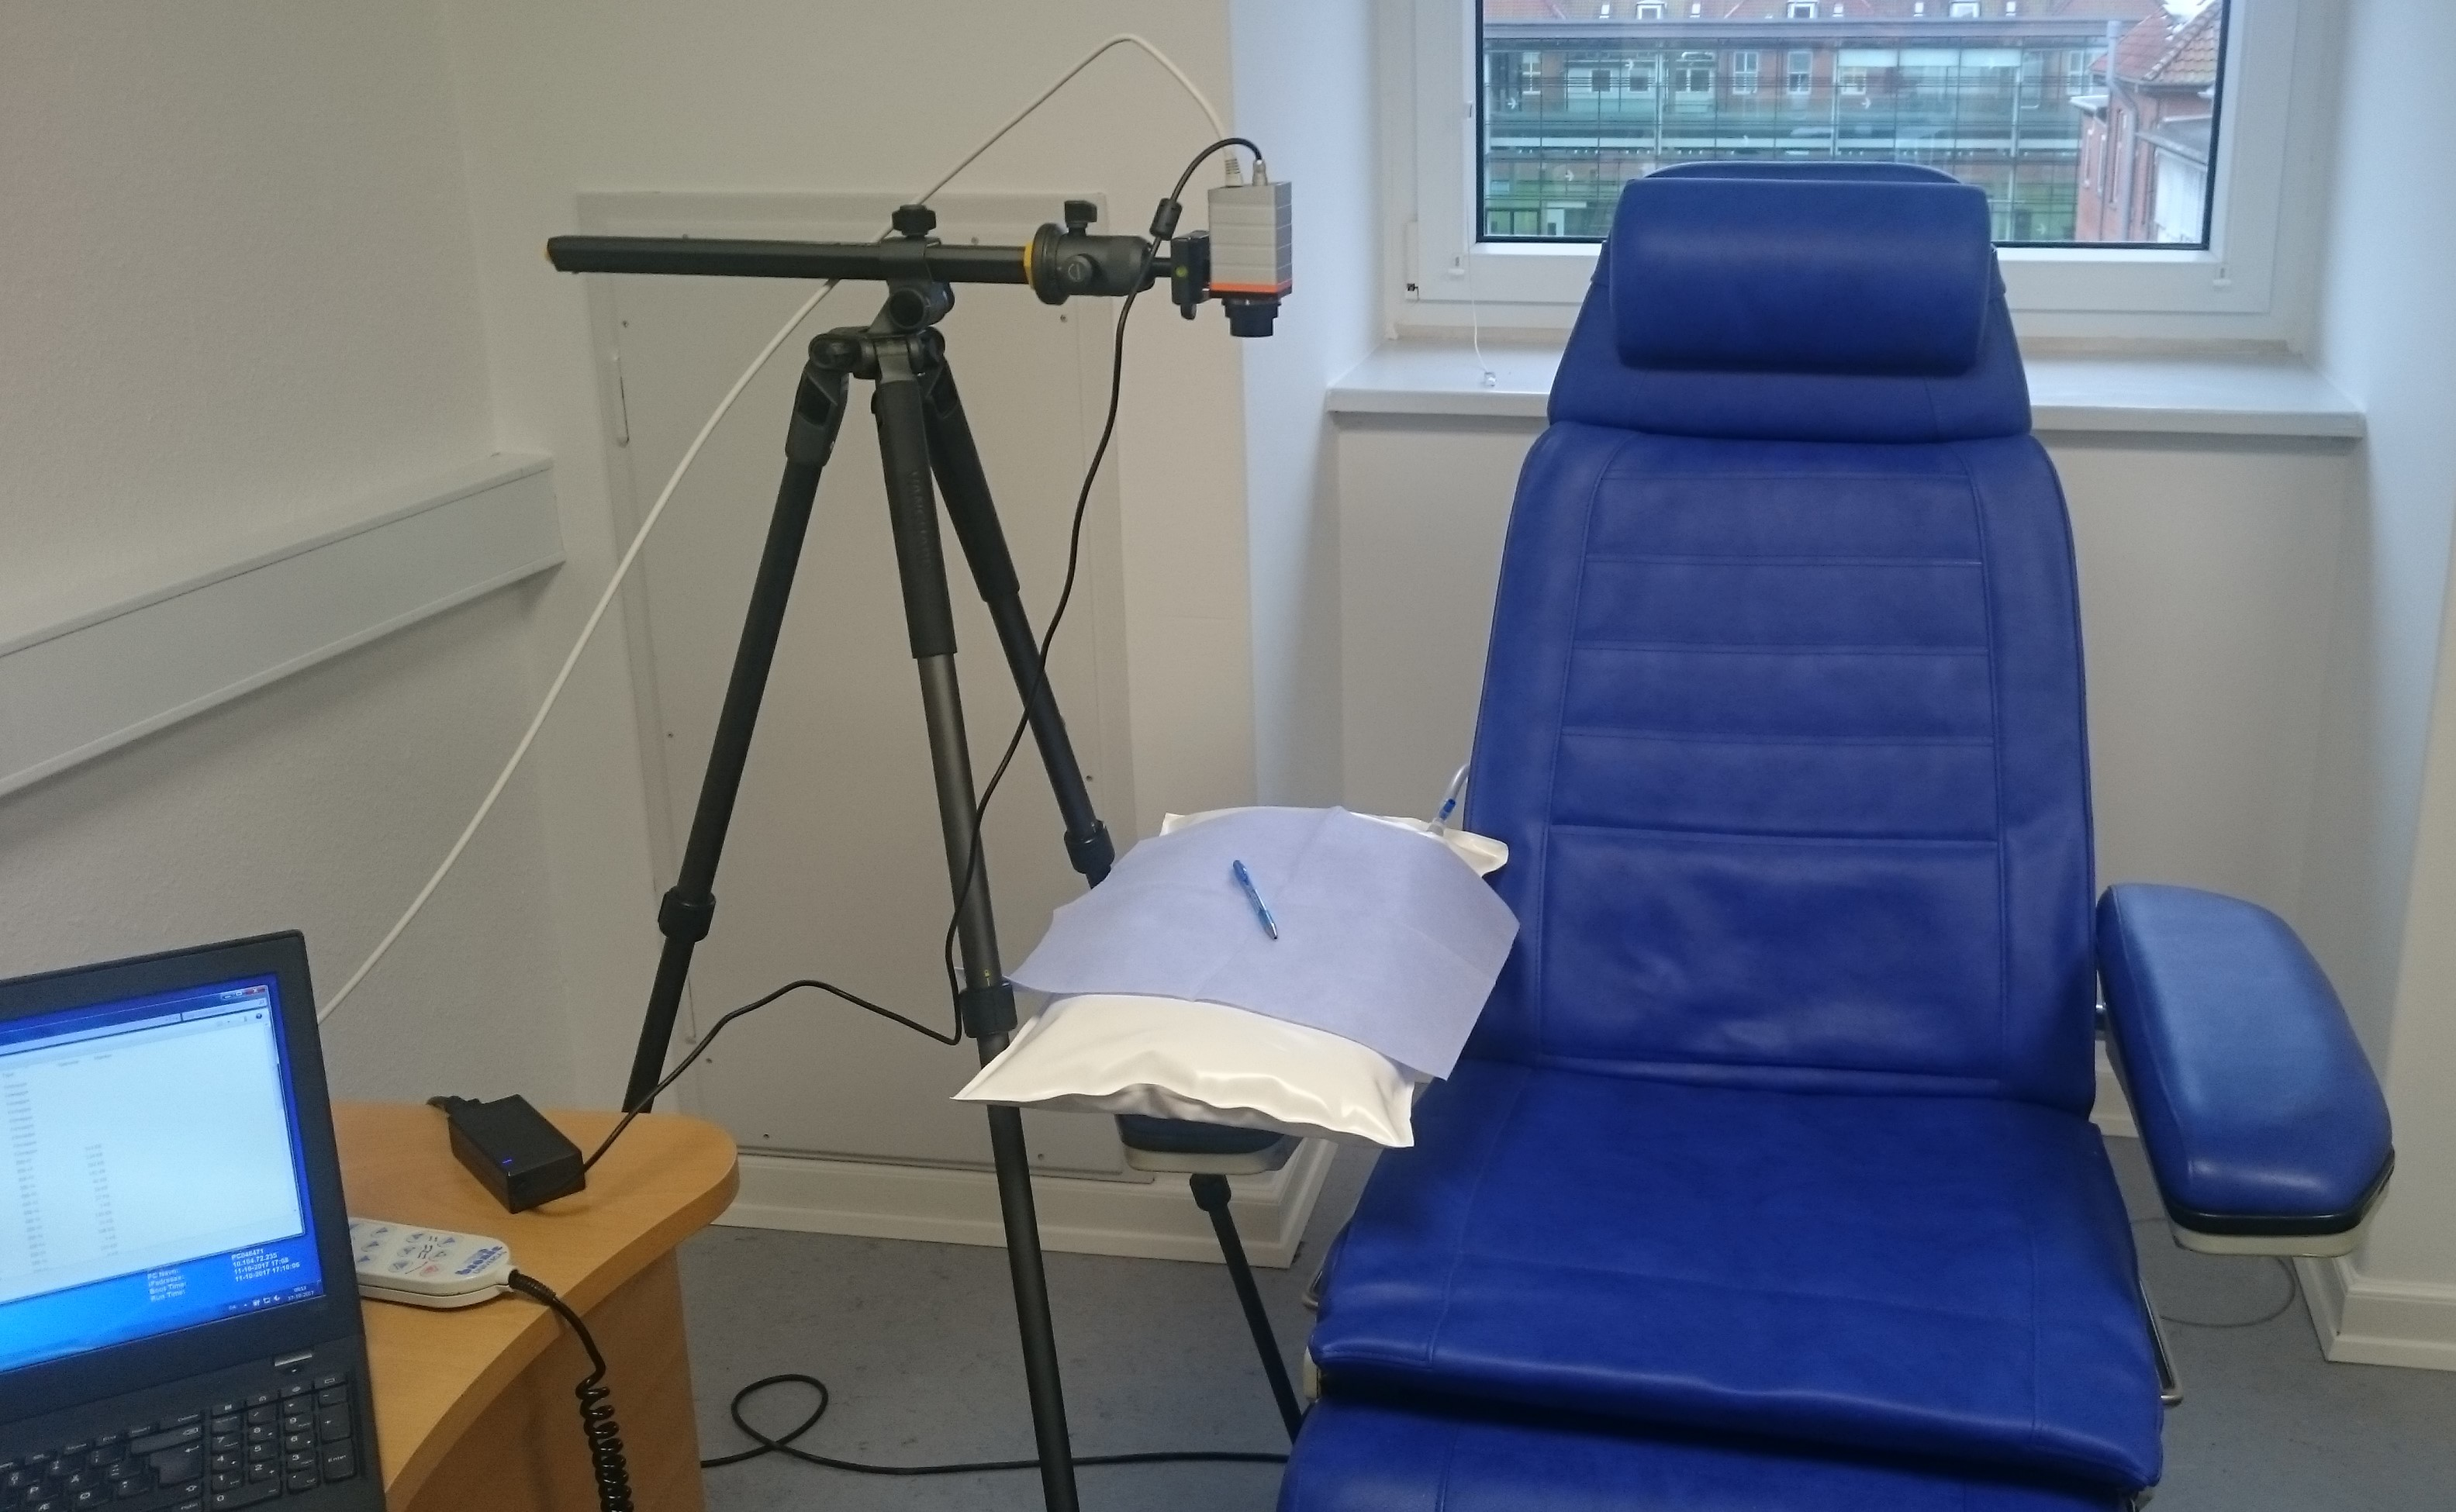
\includegraphics[width=0.7\textwidth]{figures/setting}
	\caption{The test setting at the Regionshospital Nordjylland.}
	\label{fig:setting}
\end{figure}

The camera was via a Ethernet cable connected with a laptop, which was used to record the measurements with Xeneth 2.6 software. 
First cable connections between the camera, the laptop and the power supply were set. Afterwards the camera was turned on and had to warm up for about 15 min. During this the laptop was started and the software for taking the measurements was set in operational readiness.

When the preparation of the test setting was done, the preparation for the subject begun. At first the blood pressure of the subject was measured on the dominant arm. The blood pressure was measured three times while the subject was sitting relaxed on a chair. Mean systolic blood pressures was calculated. To get the total occlusion pressure $(TOP)$ the mean was multiplied by 1.3. To reduce the blood flow in the arm to 50\% during the measurement within the second condition, the arm was cuffed with 30\% of the $TOP$.\cite{mouser2017} 
Then the cuff was affixed at the subjects dominant arm without tighten it, so that it was ready for the second part of the experiment. After that the subject took place in the chair and the hand was stabled with the vacuum pillow. The vacuum generator was attached to the pillow for giving the hand more stability. The lens focus has been adjusted so the distance was taken into consideration, to make sure the image was sharp.

When the camera was stable and the filename was modified according to the subject, the first measurement was started for 20 min. During the whole experiment the subject was not allowed to move or speak to minimize movement bias.
Directly after the first measurement the cuff on the arm of the subject was tightened with the calculated value. The pressure of the cuff had to be observed during the whole measurement and if necessary adjusted.

To guide the conductors of the experiment, an experimental protocol was formed and followed during the experiment. The experimental protocol can be seen in \cref{chap:protocol}. 

